\chapter{Methodology}\label{chapter:methodology}

\begin{figure}
	\centering
	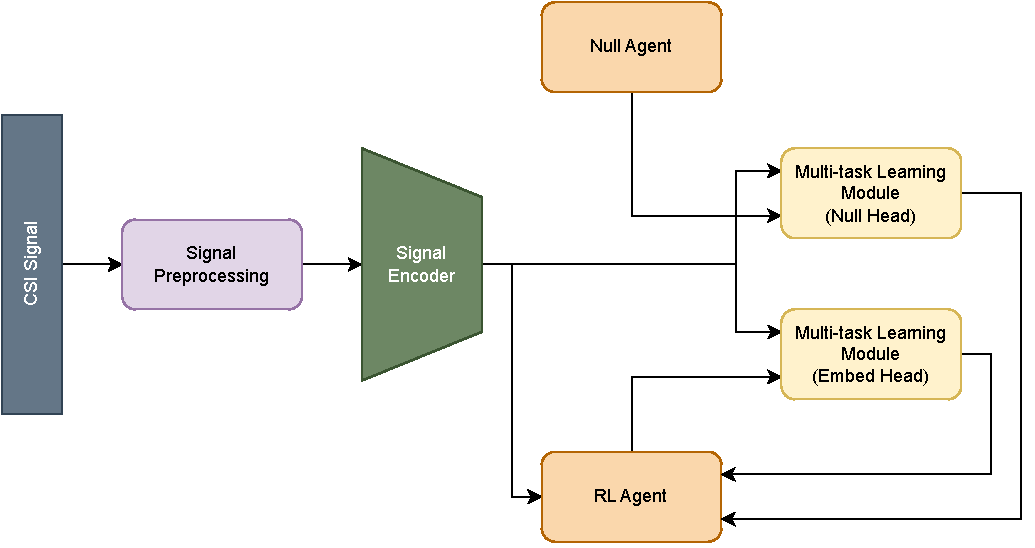
\includegraphics[width=\linewidth]{figures/arch_diagram.pdf}
	\caption{An abstracted diagram of the proposed architecture in this thesis.}
	\label{fig:arch-diagram}
\end{figure}

The general intuition behind our approach is the lack of ability for a model to perform on unseen domains without any additional information.
The general architecture of our approach can be seen in Figure \ref{fig:arch-diagram}.
We first propose a signal preprocessing and signal-to-image transformation pipeline, described in Section \ref{sec:methodology-signal-preprocessing} and \ref{sec:methodology-signal-to-image}.
This transforms the input signal into an image that is then passed through a CNN encoder, as described in Section {sec:methodology-signal-encoding}, encoding the signal into a latent representation.
This latent representation is then used in two different ways: As an input for the multi-task learning heads, described in Section \ref{sec:methodology-multi-task-learning}, and as the state observation for our RL agent, described in Section \ref{sec:methodology-rl}.

To mitigate domain-shift, our RL agent is tasked with producing the best possible embedding of the domain $D_{r}$ as its action given the signal latent representation as its state observation.

To provide the RL agent with a reward function, inspired by triplet loss, we use two different multi-task learning modules.
One of these modules is provided $D_{0}$, representing a vector of zeros, and the other $D_{r}$.

%\todonotestodo[inline]{This chapter is not finalized, due to the possibility of changing things around so will be kept as bullet points at this stage.}

\section{Signal Preprocessing}\label{sec:methodology-signal-preprocessing}

\begin{figure}
	\centering
	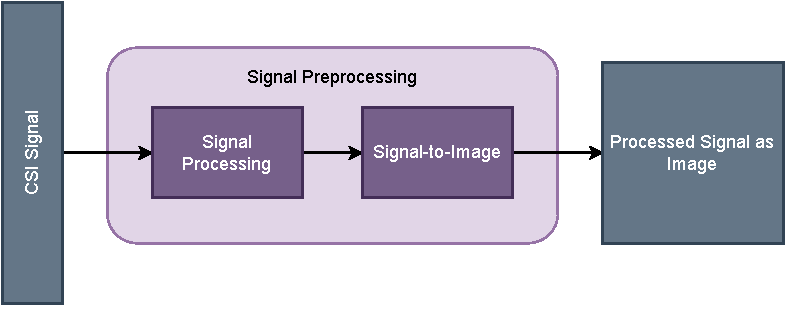
\includegraphics[width=0.8\linewidth]{figures/signal_preprocessing_diagram.pdf}
	\caption{Details of the signal preprocessing module. The module is comprised of traditional signal preprocessing and a signal-to-image transformation.}
	\label{fig:signal-preprocessing-diagram}
\end{figure}

As the old adage goes, garbage in, garbage out.
As such, we propose a signal preprocessing module, visualized in Figure \ref{fig:signal-preprocessing-diagram}.
This module first cleans the signal using traditional signal preprocessing and then transforms it into an image for use by the signal encoder.

\subsection{Signal Processing}

We propose the following steps from traditional signal processing to clean up the input signal for our ML algorithm.

\begin{itemize}
	\item Noise filtering with a low-pass filter, since high-freq noise is most likely not human movement
	\item CSI Phase unwrapping and linear fitting as suggested by \cite{geng2022densepose}
	\item CSI Phase derivative, to keep values from changing magnitude as in the case of unwrapping
	\item DWT seems to have been attempted in some papers, so let's see if that helps.
	\item We'll do an ablation study to see if these actually help
\end{itemize}

The signal can now be considered clean, or at least clean enough that we can continue with further steps.

\subsection{Signal-to-Image Transformation}\label{sec:methodology-signal-to-image}

%Four crazy signal-to-image transformation methods! You won't believe number three!\todo{If there are no objections, this will be in the final paper}

The next stage in our method is transform the signal into an image, leveraging advances from computer vision.
There are many works from the literature which show that there are certainly improvements that can be gained from performing image processing on temporal data.
We will experiment with the following four methods for signal-to-image transformation: DeepInsight \cite{sharma2019deepinsight}, REFINED \cite{bazgir2020representation}, GAF/FGAF (Feature-wise GAF) \cite{wang2015imaging,satyawan2023cnns}, and MTF \cite{wang2015imaging}.

\subsubsection{DeepInsight}

DeepInsight \cite{sharma2019deepinsight} applies t-SNE on the columns of $V$, resulting in each AP $k$ being mapped to a point in 2D space.
The entire space is then rotated to fit within the minimum rectangular bounding box.
These rotated points then become the pixel coordinates for a given AP.
The value of the RSSI of a given AP $k$ is then directly mapped to the value of its corresponding pixel.
If multiple features share a pixel location, the average value of these features is then used as the value of the pixel.

\subsubsection{REFINED}

REpresentation of Features as Images with NEighborhood Dependencies \cite{bazgir2020representation} uses a technique the authors call ``Bayesian Multidimensional Scaling''.
A 2D embedding of the data $V_{embed}$ is calculated using Multidimensional Scaling (MDS) with a Euclidean distance metric.
A pixel grid $P$ of $p^2$ pixels, where $p=\left\lceil \sqrt{K} \right\rceil$ is then produced with dimensions $p \times p$.
A mapping of features to pixels is calculated by considering all permutations which minimize the Euclidean distance of the pixel mapping to the feature location in $V_{embed}$ while keeping at most one feature per pixel iteratively.
This final mapping is calculated using a hill-climb algorithm.

\subsubsection{GAF}

Gramian Angular Fields \cite{wang2015imaging} first transform the incoming signal for each AP to polar coordinates with
\begin{equation}
	\vec{w_{i, k}} = \begin{cases}
		\phi_{i, k} = \arccos(V_{n, k}) \\
		r_{i, k} = i / I
	\end{cases}
\end{equation}
where $\vec{w_{i, k}}$ is the resulting vector of a signal, $V_{i, k}$ the value of the signal from AP $K$ at sample $i$, $i$ the sample number of the fingerprint, and $I$ the total number of timesteps at the given sample location.
For the case of our dataset, there are 6 timesteps for each location.

The Gramian is than calculated as
\begin{equation}
	G_k = \begin{bmatrix}
		w_{1,k} \cdot w_{1,k} & \cdots & w_{1,k} \cdot w_{I,k} \\
		\vdots                & \ddots & \vdots \\
		w_{I,k} \cdot w_{1,k} & \cdots & w_{I,k} \cdot w_{I,k}
	\end{bmatrix}
\end{equation}
for each AP $k$ creating an image with $k$ channels.

We discovered in a previous project that calculating vector $\vec{w}$ across features, i.e., channels, instead of across timesteps can also be useful. 
This results in
\begin{equation}
	\vec{w_{n, k}} = \begin{cases}
		\phi_{n, k} = \arccos(V_{n, k}) \\
		r_{n, k} = k / K
	\end{cases}
\end{equation}
where $n$ is the sample index and $k$ is the feature index. This leads to the Gramian for each sample 
\begin{equation}
	G_n = \begin{bmatrix}
		w_{n, 1} \cdot w_{n, 1} & \ldots & w_{n, 1} \cdot w_{n, K} \\
		\vdots                  & \ddots & \vdots \\
		w_{n, K} \cdot w_{n, 1} & \cdots & w_{n, K} \cdot w_{n, K}
	\end{bmatrix}
\end{equation}
We call this transformation Feature-wise GAF (FGAF).

In either case, $G$ is finally normalized.

\subsubsection{MTF}

Markovian Transition Fields \cite{wang2015imaging} first quantizes the signal into $q$ bins, each bin representing an interval of RSSI strength.
A Markovian transition matrix $M_{t}$ is then constructed where each row represents a fingerprint and each column a bin. 
The values in $M_{t}$ are the size of each bin for a given sample.
$M_{t}$ is then normalized and aligned along the temporal axis such that in this new matrix $M$, $M_{i, j}$ represents the probability of a transition from bin $i$ to bin $j$.
$M$ is then an image of size $q \times q$.

Regardless of the chosen method, the signal has now been transformed into an image and we can proceed with the encoding of this image into a latent space.

\section{Signal encoding}\label{sec:methodology-signal-encoding}

The encoding of the signal, now an image, into a latent space is performed using CNN-based image processing methods.

\begin{itemize}
	\item The signal encoding backbone is a standard CNN
	\item This will probably be something simple, like ResNet since the signal shouldn't be too complex that it requires something very SOTA
	\item Alternatively, mobilenet may be used as well
	\item This may actually be the least important aspect of this thesis
\end{itemize}

The latent representation of this signal is then passed to both the reinforcement learning agent as its state observation as well as to the multi-task learning modules.
How the RL agent uses this state observation is described in Section \ref{sec:methodology-rl} while its use by the multi-task learning module is described in Section \ref{sec:methodology-multi-task-learning}.

\section{Unsupervised Domain Representations through Reinforcement Learning}\label{sec:methodology-rl}

To mitigate domain shift, we implement a novel method for unsupervised domain representations through reinforcement learning.

\begin{itemize}
	\item Base terminology: Agent, action, state observation (state), and reward
	\item The encoder-decoder architecture described in Section \ref{sec:methodology-signal-encoding} and \ref{sec:methodology-multi-task-learning} is the environment.
	\item RL loop:
	\begin{enumerate}
		\item The agent receives the image embedding produced by the encoder/backbone as its state
		\item The reinforcement learning agent produces an embedding of the domain as its action
		\item The environment is trained with one pair of heads receiving the action of the agent while the other pair receives senseless values (either all 0s if the representation is one-hot or a uniform distribution if the representation is a probability measure)
		\item After training of the agent, the RL agent is provided a reward from the environment which is used to improve the agent
	\end{enumerate}
	\item Let a performance metric function $M$ denote the gesture classification performance of a multi-task learning module given the gesture classification prediction $\hat{y_{c}}$. Then, the reward function $R$ of the agent is $R\left(M\left(\hat{y}_{c,rl}, y_c\right),M\left(\hat{y}_{c,0}, y_c\right)\right)$ and calculates the gesture prediction performance difference between the module given the domain embedding and the module given the null embedding.
	\begin{itemize}
		\item The intuition is, the reward is based on how much better the head pair with the action should perform than the head pair without the action
		\item This is based on the idea behind triplet loss, where in an unsupervised scenario, model performance can be determined by the metric performance differential between two inputs. Maximizing this difference implies better total model performance.
		\item We will also experiment with L1 vs L2 regularization on the reward, representated by the function $R$.
	\end{itemize}
	\item To speed up training, we take a page from AutoML competitions and the environment is trained within 1 minute and be focused on improving performance as fast as possible instead of achieving the best performance, at least during hyperparam optimization
	\item After hyperparameters are chosen, then we train properly and fully.
	\item A reward is then calculated using the function $R\left(M\left(\hat{y}_{rl}, y\right)-M\left(\hat{y}_{0}, y\right)\right)$, where $M$ is the metric used to calculate the performance of the gesture classifier in each multi-task learning module and $R$ is some reward function.
	\item We do not use the absolute difference, as we are interested in the having negative values representing the module provided $D_0$ having better performance.
	\item We will be looking at PPO \cite{schulman2017proximal} and SARSA \cite{rummery1994line}
	\begin{itemize}
		\item We've used both these techniques before in a previous project, so implementation should be relatively straightforwards
	\end{itemize}
	\item \emph{Motivation}
	\begin{itemize}
		\item We use the RL agent inspired by \cite{ma2021location} and hypothesize that the RL architecture there can be extended to domain auto-labeling
		\item We use the triplet-loss approach since triplet loss is a proven way to provide a numerical value showing the difference between two input
		\begin{itemize}
			\item In other words, this is analogous to testing the null hypothesis, where $H_0$ is no RL agent produced domain embedding and $H_1$ is a RL agent produced domain embedding
			\item Our hypothesis is that the domain embedding will produce better results
			\item If the RL agent can be trained, then the difference $(M\left(\hat{y}_{rl}, y\right)-M\left(\hat{y}_{0}, y\right)$ will approach $M\left(\hat{y}_{rl}, y\right)$ producing the maximum reward for the RL agent
		\end{itemize}
	\end{itemize}
\end{itemize}

\section{Multi-task Learning}\label{sec:methodology-multi-task-learning}

\begin{figure}
	\centering
	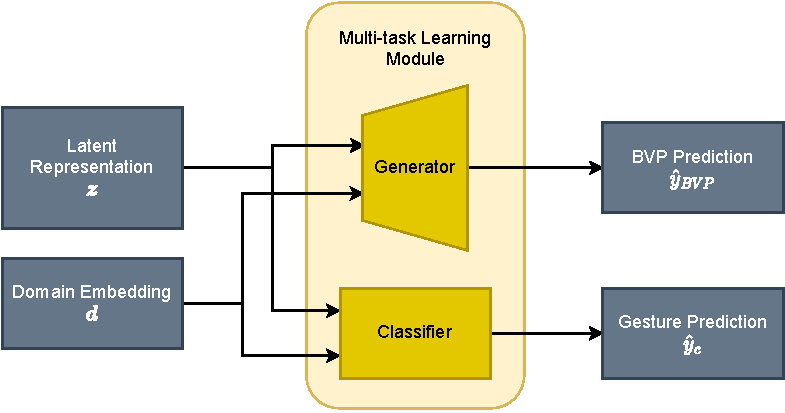
\includegraphics[width=0.8\linewidth]{figures/multitask_learning_module_diagram.pdf}
	\caption{Details of the multi-task learning module. The generator is made up of a series of deconvolutional layers and produces the BVP prediction while the classifier is a fully connected network and produces a probability distribution over each gesture class.}
	\label{fig:multitask-learning-module-diagram}
\end{figure}

The actual gesture classification module is built using a multi-task learning module, a visualization of which can be seen in Figure \ref{fig:multitask-learning-module-diagram}.

\begin{itemize}
	\item The idea is to enforce some sort of representation that \textit{can} be used to get a domain-independent representation of the data
	\item We utilize multi-task learning for this, where one head is used to predict BVP, which is theoretically domain-independent \cite{zheng2019zero}
	\begin{itemize}
		\item We are not actually interested in the BVP, but having it as part of our training will enforce the need for a representation which is theoretically domain-independent.
		\item \cite{martini2021domain} suggests the use of MMD and an adversarial approach to training the model to ensure that while the representation is domain-invariant, it still retains enough discriminatory powers such that the domain classifier can still perform.
		\item Instead of this approach, we use the BVP prediction to enforce a representation which is domain-invariant and we use an RL agent instead of the domain classifier suggested in \cite{martini2021domain}.
	\end{itemize}
	\item The other head is a classifier head and classifies gestures
	\item It's been shown that doing multi-task learning like this leads to good results with latent representations which are more robust \cite{tuggener2021deepscoresv2}
	\item We duplicate this pair of heads to enable a reward function for the RL agent inspired by triplet loss
	\item Loss function for the gesture classifier is cross entropy loss
	\item Loss function for the BVP generator is cross entropy loss on the produced image.
	\item \emph{Motivation}
	\begin{itemize}
		\item We use multi-task learning since its been shown that multitask learning can produce better/more powerful/more robust/more efficient latent representations due to the latent representation being used for multiple tasks
		\item For this multi-task objective, we use BVP as the target of the generator, since we have ground-truth BVP data and \cite{zheng2019zero} makes a point to show that BVP is domain-independent
		\begin{itemize}
			\item Therfore, if the generator can produce a BVP close to the ground-truth, then we have a latent representation that can be used to produce domain-independent features
		\end{itemize}
		\item We want try to get a latent representation capable of producing domain-independent features but we don't want to enforce it directly on the latent representation, since this may not work well \cite{van2022insights} and \cite{martini2021domain} suggests giving the representation some discriminatory abilities w.r.t. the domain.
		\begin{itemize}
			\item Therefore, we believe that enforcing domain independence on the output will result in a representation that is domain-independent enough yet still retain discriminatory power.
		\end{itemize}
		\item Cross Entropy loss on the produced image is used since it is the appropriate loss function for image generation (i.e., pixel-wise feature value prediction)
		\item We use gesture as the target of the classifier, since that's the goal of this thesis
		\item Cross Entropy loss on the prediction is used since it is the appropriate loss function for a multi-class prediction task.
		
	\end{itemize}
\end{itemize}
